\section{Text Frames}
\label{sec:textframes}
The tasks of text frames are text rendering and user interaction. A text frame represents a text view
and a controller in the form of an interactive text editor. Technically, text frames are a subclass of
display frames and, as such, are objects with an open message interface of the kind explained in
Chapter 4.

The geometric layout of text frames is determined by two areas: A rectangle of contents and a
vertical scroll-bar along the left borderline. The type of text frames is a direct extension of type
Display.Frame:
\begin{verbatim}
Frame = POINTER TO FrameDesc;
FrameDesc = RECORD (Display.FrameDesc)
text: Texts.Text;
org, col, lsp: INT;
left, right, top, bot: INT;
markH, time: INT;
hasCar, hasSel, hasMark: BOOL;
carloc: Location;
selbeg, selend: Location
END;
\end{verbatim}

Fields text and org specify the text part to be displayed, the former referring to the underlying text
and the latter designating the starting position of the displayed part. Fields col and lsp are rendering
parameters. They specify the frame's background color and the line spacing. Fields left, right, top,
and bot are margins. They determine the rectangle of contents. mark indicates whether there is a
position marker, which is a small horizontal bar indicating the position of the displayed part relative
to the whole text. markH represents its location within the text frame.

Caret and selection are two important features associated with a text frame. The caret indicates a
focus, and it serves as an implicit "point of insertion" for placing consumed characters (for example
from the keyboard). The selection is a stretch of displayed text. Additionally it serves as a
parameter for various operations and commands, among them delete and change looks. The state
and location of the caret is given by the variables car and carloc respectively. Analogously, the
state of the selection and its begin and end are reflected by the fields sel, selbeg, and selend in the
frame descriptor. Field time is a time stamp on the current selection.

In principle, caret and selection could be regarded as ingredients of the underlying text (the model)
equally well. However, we deliberately decided to associate these features with frames (views) in
order to get increased flexibility. For example, two different selections in adjacent viewers
displaying the same text are normally interpreted as one extensive selection across their span.
The auxiliary type Location summarizes information about a location in a text frame. Its definition is:
\begin{verbatim}
Location = RECORD
org, pos, dx, x, y: INT
END;
\end{verbatim}

x, y specify the envisioned location relative to the text frame's origin, and dx is the width of the
character at this location. pos is the corresponding position in the text and org is the origin position
of the corresponding text line.

The following is a simplified version of the message handler employed by text frames. It fully
determines the behavior and capabilities of text frames.
\begin{verbatim}

1)
2)

3)
4)
5)
7)
8)
9)

PROC Handle* (F: Display.Frame; VAR M: Display.FrameMsg);
VAR F1: Frame; buf: Texts.Buffer;
BEGIN
CASE M OF
Oberon.InputMsg:
IF M.id = Oberon.track THEN Edit(F(Frame), M.X, M.Y, M.keys)
ELSIF M.id = Oberon.consume THEN
IF F(Frame).hasCar THEN Write(F(Frame), M.ch, M.fnt, M.col, M.voff) END
END |
Oberon.ControlMsg:
IF M.id = Oberon.defocus THEN Defocus(F(Frame))
ELSIF M.id = Oberon.neutralize THEN Neutralize(F(Frame))
END |
Oberon.SelectionMsg:
GetSelection(F(Frame), M.text, M.beg, M.end, M.time) |
Oberon.CopyMsg: Copy(F(Frame), F1); M.F := F1 |
MenuViewers.ModifyMsg: Modify(F(Frame), M.id, M.dY, M.Y, M.H) |
CopyOverMsg: CopyOver(F(Frame), M.text, M.beg, M.end) |
UpdateMsg: IF F(Frame).text = M.text THEN Update(F(Frame), M) END
END
END Handle;
\end{verbatim}

Explanations:
1)
2)
3)
4)
5)
6)
7)
8)
9)

Mouse tracking message: Call built-in editor immediately
Consume message: In case of valid caret insert character
Defocus message: Remove caret
Neutralize message: Remove caret and selection
Selection message: Return current selection with time stamp
Copyover message: Copy given stretch of text to caret
Copy message: Create a copy (clone)
Modify message: Translate and change size
Update message: If text was changed then update display

We recognize again our categories of universal messages introduced in Chapter 4, Table 4.6:
Messages in lines 1) and 2) report about user interactions. Messages in 3), 4), 5), 6), and 7) specify
generic operations. Messages in 8) require a change of location or size. Messages of the latter kind
arrive from the ancestor menu viewer via delegation. They are generated by the interaction handler
and preprocessed by the original viewer message handler. Finally, messages in line 9) report about
changes of contents.

The text frame handler is encapsulated in a module called TextFrames. This module exports the
above introduced types Frame (text frame) and Location, as well as the procedure Handle.
Furthermore, it exports type UpdateMsg to report on changes made to a displayable text.
\begin{verbatim}
UpdateMsg = RECORD (Display.FrameMsg)
id: INT;
text: Texts.Text;
beg, end: INT
END;
\end{verbatim}

Field id names one of the operators replace, insert, or delete. The remaining fields text, beg, and
end restrict the change to a range. Additional procedures generate a new standard menu text frame
and contents text frame respectively:
\begin{verbatim}
PROC NewMenu (name, commands: ARRAY OF CHAR): Frame;
PROC NewText (text: Texts.Text; pos: INT): Frame;
\end{verbatim}

This completes the minimum definition of module TextFrames. In addition, this module exports a
set of useful service procedures supporting the composition of custom handlers from elements of
the standard handler:
\begin{verbatim}
PROC Edit (F: Frame; X, Y: INT; Keys: SET);
PROC Write (F: Frame; ch: CHAR; fnt: Fonts.Font; col, voff: INT);
PROC Defocus (F: Frame);
PROC Neutralize (F: Frame);
PROC GetSelection (F: Frame; VAR text: Texts.Text;
VAR beg, end, time: INT);
PROC CopyOver (F: Frame; text: Texts.Text; beg, end: INT);
PROC Copy (F: Frame; VAR F1: Frame);
PROC Modify (F: Frame; id, dY, Y, H: INT);
PROC Update (F: Frame; VAR M: UpdateMsg);
\end{verbatim}

The module also supports mouse tracking inside text frames:
\begin{verbatim}
PROC TrackCaret (F: Frame; X, Y: INT; VAR keysum: SET);
PROC TrackSelection (F: Frame; X, Y: INT; VAR keysum: SET);
PROC TrackLine (F: Frame; X, Y: INT; VAR org: INT; VAR keysum: SET);
PROC TrackWord (F: Frame; X, Y: INT; VAR pos: INT; VAR keysum: SET);
\end{verbatim}

Let us now take a closer look at the implementation of some selected operations. For this purpose,
we must first explain the notion of line descriptor that is used to optimize the operation of locating
positions within text frames.
\begin{verbatim}
Line = POINTER TO LineDesc;
LineDesc = RECORD
len, wid: INT;
eot: BOOL;
next: Line
END;
\end{verbatim}

Each line descriptor provides detailed information about a single line of text that is currently
displayed: len is the number of characters on the line, wid is the line width, eot indicates
terminating line, and next points to the next line descriptor.

Text frames maintain a private data structure called line list that describes the list of text lines
displayed:
\begin{verbatim}
Frame = POINTER TO FrameDesc;
FrameDesc = RECORD (Display.FrameDesc)
text: Texts.Text;
org, col, lsp: INT;
left, right, top, bot: INT;
markH, time: INT;
hasChar, hasSel, hasMark: BOOL;
carloc, selbeg, selend: Location;
--> trailer: Line
END;
\end{verbatim}

Field trailer represents a sentinel element that closes the line list to a ring.
The line list contains useful summary information about the current contents of the text frame. It can
be used beneficially by some related data types, for example by type Location that was introduced
earlier:
\begin{verbatim}
Location = RECORD
org, pos, dx, x, y: INT;
--> lin: Line
END;
\end{verbatim}

The built-in editor procedure Edit is a worthwhile part to look at in more detail. It is called by the task
scheduler to handle mouse events within a text frame. The following code excerpt shows nicely
how the different components of the text system interoperate.
\begin{verbatim}
PROC Edit* (F: Frame; X, Y: INT; Keys: SET);
VAR M: CopyOverMsg;
text: Texts.Text;
buf: Texts.Buffer;
v: Viewers.Viewer;
loc0, loc1: Location;
beg, end, time, pos: INT;
keysum: SET;
fnt: Fonts.Font;
col, voff: INT;
BEGIN
IF X < F.X + Min(F.left, barW) THEN (*cursor is in scroll bar*)
Oberon.DrawMouse(ScrollMarker, X, Y); keysum := Keys;
IF Keys = {2} THEN (*ML, scroll up*)
TrackLine(F, X, Y, pos, keysum);
IF (pos >= 0) & (keysum = {2}) THEN
RemoveMarks(F); Oberon.RemoveMarks(F.X, F.Y, F.W, F.H);
Show(F, pos)
END
ELSIF Keys = {1} THEN (*MM*) keysum := Keys;
REPEAT Input.Mouse(Keys, X, Y); keysum := keysum + Keys;
Oberon.DrawMouse(ScrollMarker, X, Y)
UNTIL Keys = {};
IF ~(keysum = {0, 1, 2}) THEN
IF 0 IN keysum THEN pos := 0
ELSIF 2 IN keysum THEN pos := F.text.len - 100
ELSE pos := (F.Y + F.H - Y) * (F.text.len) DIV F.H
END ;
RemoveMarks(F); Oberon.RemoveMarks(F.X, F.Y, F.W, F.H);
Show(F, pos)
END
ELSIF Keys = {0} THEN (*MR, scroll down*)
TrackLine(F, X, Y, pos, keysum);
IF keysum = {0} THEN
LocateLine(F, Y, loc0); LocateLine(F, F.Y, loc1);
pos := F.org - loc1.org + loc0.org;
IF pos < 0 THEN pos := 0 END ;
RemoveMarks(F); Oberon.RemoveMarks(F.X, F.Y, F.W, F.H);
Show(F, pos)
END
END
ELSE (*cursor is in text area*)
Oberon.DrawMouseArrow(X, Y);
IF 0 IN Keys THEN (*MR: select*)
TrackSelection(F, X, Y, keysum);
IF F.hasSel THEN
IF keysum = {0, 2} THEN (*MR, ML: delete text*)
Oberon.GetSelection(text, beg, end, time);
Texts.Delete(text, beg, end, TBuf);
Oberon.PassFocus(Viewers.This(F.X, F.Y)); SetCaret(F, beg)
ELSIF keysum = {0, 1} THEN (*MR, MM: copy to caret*)
Oberon.GetSelection(text, beg, end, time);
M.text := text; M.beg := beg; M.end := end;
Oberon.FocusViewer.handle(Oberon.FocusViewer, M)
END
END
ELSIF 1 IN Keys THEN (*MM: call*)
TrackWord(F, X, Y, pos, keysum);
IF (pos >= 0) & ~(0 IN keysum) THEN Call(F, pos, 2 IN keysum) END
ELSIF 2 IN Keys THEN (*ML: set caret*)
Oberon.PassFocus(Viewers.This(F.X, F.Y));
TrackCaret(F, X, Y, keysum);
IF keysum = {2, 1} THEN (*ML, MM: copy from selection to caret*)
Oberon.GetSelection(text, beg, end, time);
IF time >= 0 THEN
NEW(TBuf); Texts.OpenBuf(TBuf);
Texts.Save(text, beg, end, TBuf); Texts.Insert(F.text, F.carloc.pos, TBuf);
SetSelection(F, F.carloc.pos, F.carloc.pos + (end - beg));
SetCaret(F, F.carloc.pos + (end - beg))
ELSIF TBuf # NIL THEN
NEW(buf); Texts.OpenBuf(buf);
Texts.Copy(TBuf, buf); Texts.Insert(F.text, F.carloc.pos, buf);
SetCaret(F, F.carloc.pos + buf.len)
END
ELSIF keysum = {2, 0} THEN (*ML, MR: copy looks*)
Oberon.GetSelection(text, beg, end, time);
IF time >= 0 THEN
Texts.Attributes(F.text, F.carloc.pos, fnt, col, voff);
IF fnt # NIL THEN Texts.ChangeLooks(text, beg, end, {0,1,2}, fnt, col, voff) END
END
END
END
END
END Edit;
\end{verbatim}

We see that the editing operation is determined by the first key pressed (primary key) and can then
be varied by “interclicking” that is, by clicking a secondary key while holding down the primary key.
As a convention, (inter)clicking all keys means cancelling the operation. Mouse clicks and
subsequent actions can now be summarized as follows:
1. In the scroll bar
primary key

secondary key

action

ML
MM
MM
MM

ML
MR

scroll designated line to the top
scroll proportional to mouse position
scroll to the end of the text
scroll to the beginning of the text

primary key

secondary key

action

ML
ML
ML
MM
MR
MR
MR

MM
MT
ML
MM

set caret
copy selection to caret
copy looks
call selected procedure
select
delete selection
copy selection to caret

2. In the text area
In the text area the keys are interpreted according to their generic semantics:
left key =
middle key =
right key =

point key
execute key
select key

Let us “zoom into” one of the editing operations, for example into TrackCaret.
\begin{verbatim}
PROC TrackCaret (F: Frame; X, Y: INT; VAR keysum: SET);
VAR loc: Location; keys: SET;
BEGIN
1) IF F.trailer.next # F.trailer THEN
2)
LocateChar(F, X - F.X, Y - F.Y, F.carloc);
3)
FlipCaret(F);
4)
keysum := {};
REPEAT
Input.Mouse(keys, X, Y); keysum := keysum + keys;
Oberon.DrawMouseArrow(X, Y);
LocateChar(F, X - F.X, Y - F.Y, loc);
IF loc.pos # F.carloc.pos THEN FlipCaret(F); F.carloc := loc; FlipCaret(F) END
5)
UNTIL keys = {};
6)
F.hascar := TRUE
END
END TrackCaret;
\end{verbatim}

Explanations:
1) guard guarantees non-empty line list
2) locates the character pointed at
3) drags caret to new location
4) - 5) tracks mouse and drags caret accordingly
6) set caret state
TrackCaret makes use of two auxiliary procedures FlipCaret and LocateChar. FlipCaret is used to
turn off or on the pattern of the caret. LocateChar is an important operation that is used to locate
the character at a given Cartesian position (x, y) within the frame.
\begin{verbatim}
PROC FlipCaret (F: Frame);
BEGIN
1) IF F.carloc.x < F.W THEN
2)
IF (F.carloc.y >= 10) & (F.carloc.x + 12 < F.W) THEN
3)
Display.CopyPattern(Display.white, Display.hook,
F.X + F.carloc.x, F.Y + F.carloc.y - 8, Display.invert)
END
END
END FlipCaret;
\end{verbatim}

Explanations:
1) - 2) if there is room for drawing the caret
3) copy standard hook-shaped pattern to caret location in inverse video mode
\begin{verbatim}
PROC LocateChar (F: Frame; x, y: INT; VAR loc: Location);
VAR R: Texts.Reader;
patadr, pos, lim: INT;
ox, dx, u, v, w, h: INT;
1) BEGIN LocateLine(F, y, loc);
2) lim := loc.org + loc.lin.len - 1;
3) pos := loc.org; ox := F.left; dx := eolW;
4) Texts.OpenReader(R, F.text, loc.org);
5) WHILE pos # lim DO
6)
Texts.Read(R, nextCh);
7)
Fonts.GetPat(R.fnt.raster, nextCh, dx, u, v, w, h, patadr);
IF ox + dx <= x THEN
INC(pos); ox := ox + dx;
IF pos = lim THEN dx := eolW END
ELSE lim := pos
END
END ;
8) loc.pos := pos; loc.dx := dx; loc.x := ox
END LocateChar;
\end{verbatim}
Explanations:
1) locate text line corresponding to at y
2) set limit to the last actual character on this line
3) start locating loop with first character on this line
4) setup reader and read first character of this line
5) - 7) scan through characters of this line until limit or x is reached
6) get character width dx of current character
8) return location found
Note that the need to read characters from the text (again) in LocateChar has its roots in the socalled proportional fonts in which our rich texts are represented. We found that keeping character
widths is an unnecessary optimization thanks to the buffering capabilities of the underlying file
system. In the case of fixed-pitch fonts a simple division by the character width would be sufficient,
of course.
Finally, procedure LocateLine uses the line list to locate the desired text line without reading text at
all.
\begin{verbatim}
PROC LocateLine (F: Frame; y: INT; VAR loc: Location);
VAR L: Line; org, cury: INT;
BEGIN org := F.org;
1) org := F.org; L := F.trailer.next; cury := F.H - F.top - asr;
2) WHILE (L.next # F.trailer) & (cury > y + dsr) DO
org := org + L.len; L := L.next; cury := cury - lsp
3) END;
4) loc.org := org; loc.lin := L; loc.y := cury
END LocateLine;
\end{verbatim}

Explanations:
1) start with first line in the frame
2) - 3) traverse line chain until last line or y is reached
4) return found line
After text editing text, rendering is our next topic. Let us pursue the case in that a user pressed the
point-key and then interclicked the middle key, corresponding to line 56) in procedure Edit.
Remember that notifier is called at the end of every editing operation and in particular at the end of
Texts.Insert. In case of standard text frames, the notifier simply broadcasts an update message into
the display space:
\begin{verbatim}
PROC NotifyDisplay (T: Texts.Text; op, beg, end: INT);
VAR M: UpdateMsg;
BEGIN M.id := op; M.text := T; M.beg := beg; M.end := end; Viewers.Broadcast(M)
END NotifyDisplay;
\end{verbatim}

Let us now take the perspective of a text frame receiving an update message. Looking at line 9) in
the text frame handler, we see that procedure Update is called, which in turn calls procedure Insert
in TextFrames:
\begin{verbatim}
PROC Insert (F: Frame; beg, end: INT);
VAR R: Texts.Reader; L, L0, l: Line;
org, len, curY, botY, Y0, Y1, Y2, dY, wid: INT;
BEGIN
IF beg < F.org THEN F.org := F.org + (end - beg)
ELSE
1)
org := F.org; L := F.trailer.next; curY := F.Y + F.H - F.top - asr;
WHILE (L # F.trailer) & (org + L.len <= beg) DO
org := org + L.len; L := L.next; curY := curY - lsp
2)
END;
3)
IF L # F.trailer THEN
botY := F.Y + F.bot + dsr;
4)
Texts.OpenReader(R, F.text, org); Texts.Read(R, nextCh);
5)
len := beg - org; wid := Width(R, len);
6)
ReplConst (F.col, F, F.X + F.left + wid, curY - dsr, L.wid - wid, lsp, 0);
7)
DisplayLine(F, L, R, F.X + F.left + wid, curY, len);
8)
org := org + L.len; curY := curY - lsp;
Y0 := curY; L0 := L.next;
WHILE (org <= end) & (curY >= botY) DO
NEW(l);
Display.ReplConst(F.col, F.X + F.left, curY - dsr, F.W - F.left, lsp, 0);
DisplayLine(F, l, R, F.X + F.left, curY, 0);
L.next := l; L := l;
org := org + L.len; curY := curY - lsp
9)
END;
10)
IF L0 # L.next THEN Y1 := curY;
11)
L.next := L0;
WHILE (L.next # F.trailer) & (curY >= botY) DO
L := L.next; curY := curY - lsp
12)
END;
L.next := F.trailer;
dY := Y0 - Y1;
IF Y1 > curY + dY THEN
13)
Display.CopyBlock
(F.X + F.left, curY + dY + lsp - dsr, F.W - F.left, Y1 - curY - dY,
F.X + F.left, curY + lsp - dsr,
0);
Y2 := Y1 - dY
ELSE Y2 := curY
END;
14)
curY := Y1; L := L0;
WHILE curY # Y2 DO
Display.ReplConst(F.col, F.X + F.left, curY - dsr, F.W - F.left, lsp, 0);
DisplayLine(F, L, R, F.X + F.left, curY, 0);
L := L.next; curY := curY - lsp
15)
END
END
END
END;
16) UpdateMark(F)
END Insert;
\end{verbatim}

Some explanations:
1) - 2) search line where inserted part starts
3) if it is displayed in this viewer
4) setup reader on this line
5) get width of unaffected part of line (avoid touching it)
6) clear remaining part of line
7) display new remaining part of line
8) - 9) display newly inserted text lines
10) if it was not a one line update
11) - 12) skip overwritten text lines
13) use fast block move to adjust reusable lines
14) - 15) redisplay previously overwritten text lines
16) adjust position marker

Special care needs to be exercised in the implementation to avoid "flickering" and to minimize
processing time. Concretely, the following measures are taken for this purpose:
1.) Avoid writing the same data again.
2.) Keep the number of newly rendered text lines at a minimum.
3.) Use raster operations (block moves) to adjust reusable displayed lines.

Of course, the rules governing the rendering and formatting process crucially influence the
complexity of procedures like Insert. For text frames we have consciously chosen the simplest
possible set of formatting rules. They can be summarized as:
1.) For a given text frame the distance between lines is constant.
2.) There are no implicit line breaks.

It is exactly this set of rules that makes it possible to display a text line in one pass. Two passes are
inevitable if line distances have to adjust to font sizes or if lines must be broken implicitly.
Updating algorithms make use of the following one-pass rendering procedures Width and
DisplayLine:
\begin{verbatim}
PROC Width (VAR R: Texts.Reader; len: INT): INT;
VAR patadr, pos, ox, dx, x, y, w, h: INT;
1) BEGIN pos := 0; ox := 0;
WHILE pos < len DO
Fonts.GetPat(R.fnt, nextCh, dx, x, y, w, h, pat);
ox := ox + dx; INC(pos); Texts.Read(R, nextCh)
2) END;
3) RETURN ox
END Width;
\end{verbatim}

Explanations:
1) - 2) scan through len characters of this line
3) return accumulated width
Procedures Width and LocateChar are similar. Therefore the above comment about relying on the
buffering capabilities of the underlying FS applies to procedure Width equally well.
\begin{verbatim}
PROC DisplayLine (F: Frame; L: Line;
VAR R: Texts.Reader; X, Y, len : INT);
VAR patadr; NX, Xlim, dx, x, y, w, h: INT;
1) BEGIN NX := F.X + F.W; Xlim := NX - 40;
2) WHILE (nextCh # CR) & ((nextCh > " ") OR (X < Xlim)) & (R.fnt # NIL) DO
3)
Fonts.GetPat(R.fnt, nextCh, dx, x, y, w, h, patadr);
4)
IF (X + x + w <= NX) & (h # 0) THEN
5)
Display.CopyPattern(R.col, patadr, X + x, Y + y, Display.invert)
6)
END;
7)
X := X + dx; INC(len); Texts.Read(R, nextCh)
8) END;
9) L.len := len + 1; L.wid := X + eolW - (F.X + F.left);
10) L.eot := R.fnt = NIL; Texts.Read(R, nextCh)
END DisplayLine;
\end{verbatim}

Explanations:
1) set right margin
2) - 8) display characters of this line
3) get width dx, box x, y, w, h, and pattern address of next character
4) if there is enough space in the rectangle of contents
5) display pattern
7) jump to location of next character; read next character
9) - 10) setup line descriptor

Procedure DisplayLine is again similar to LocateChar, and the comment about relying on the file
system’s buffering capabilities applies once more. The principal difference between LocateChar
and Width on one hand and DisplayLine on the other hand is the fact that the latter accesses the
display screen physically. Therefore, possession of the screen lock is a tacit precondition for calling
DisplayLine.

A quick look at an auxiliary procedure that updates the position marker concludes our tour behind
the scenes of the text system:
\begin{verbatim}
PROC UpdateMark (F: Frame);
VAR oldH: INT;
BEGIN
1) oldH := F.markH; F.markH := F.org * F.H DIV (F.text.len + 1));
IF (F.mark > 0) & (F.left >= barW) & (F.markH # oldH) THEN
2)
Display.ReplConst(Display.white, F.X + 1, F.Y + F.H - 1 - oldH, markW, 1, Display.invert);
3)
Display.ReplConst(Display.white, F.X + 1, F.Y + F.H - 1 - F.markH, markW, 1, Display.invert)
END
END UpdateMark;
\end{verbatim}

Explanations
1) shows how the marker's position is calculated. Loosely spoken, the invariant is
distance from top of frame / frame height = text position of first character in frame / text length
2) erase the old marker
3) draw the new marker

And this in turn concludes our Section on text frames. Recapitulating the most important points: The
tasks of text editing (input oriented) and text rendering (output oriented) are combined in the
concept of text frames. Text frames constitute a subclass of display frames, and they are
implemented in a separate module called TextFrames. The implementation of TextFrames
accesses the displayed text exclusively via the “official” abstract interface of module Texts
discussed in Section 5.2. It maintains a private data structure of line lists to accelerate locating
requests. Text frames use simple formatting rules that allow super-efficient rendering of text in a
single pass. In particular, line spacing is fixed for every text frame. Therefore, different styles of a
base font are possible within a given text frame while different sizes are not.

Putting into relation the different extensions of type Display.Frame that we came across in Chapters
4 and 5, we obtain the type hierarchy as shown in Fig \ref{fig:extensions}.
\begin{figure}
  \label{fig:extensions}
  \centering
  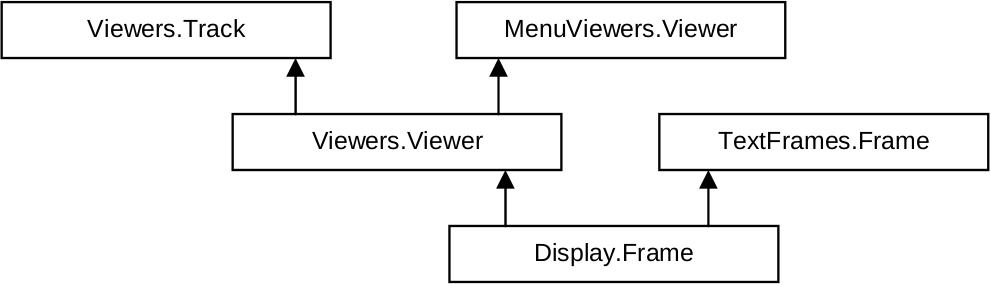
\includegraphics[width=\textwidth]{i/h}
  \caption{Extensions of type \verb|Display.Frame|}
\end{figure}


